\task{Игры}
\begin{enumerate}
\itA Двое по очереди вырезают из клетчатого прямоугольника $5 \times 2018$ фигуру, изображённую на рисунке 3{\it(a)}~— при этом её можно отражать и вращать. Проигрывает тот, кто не может вырезать фигуру в очередной раз. У кого из игроков есть выигрышная стратегия?

\centerline{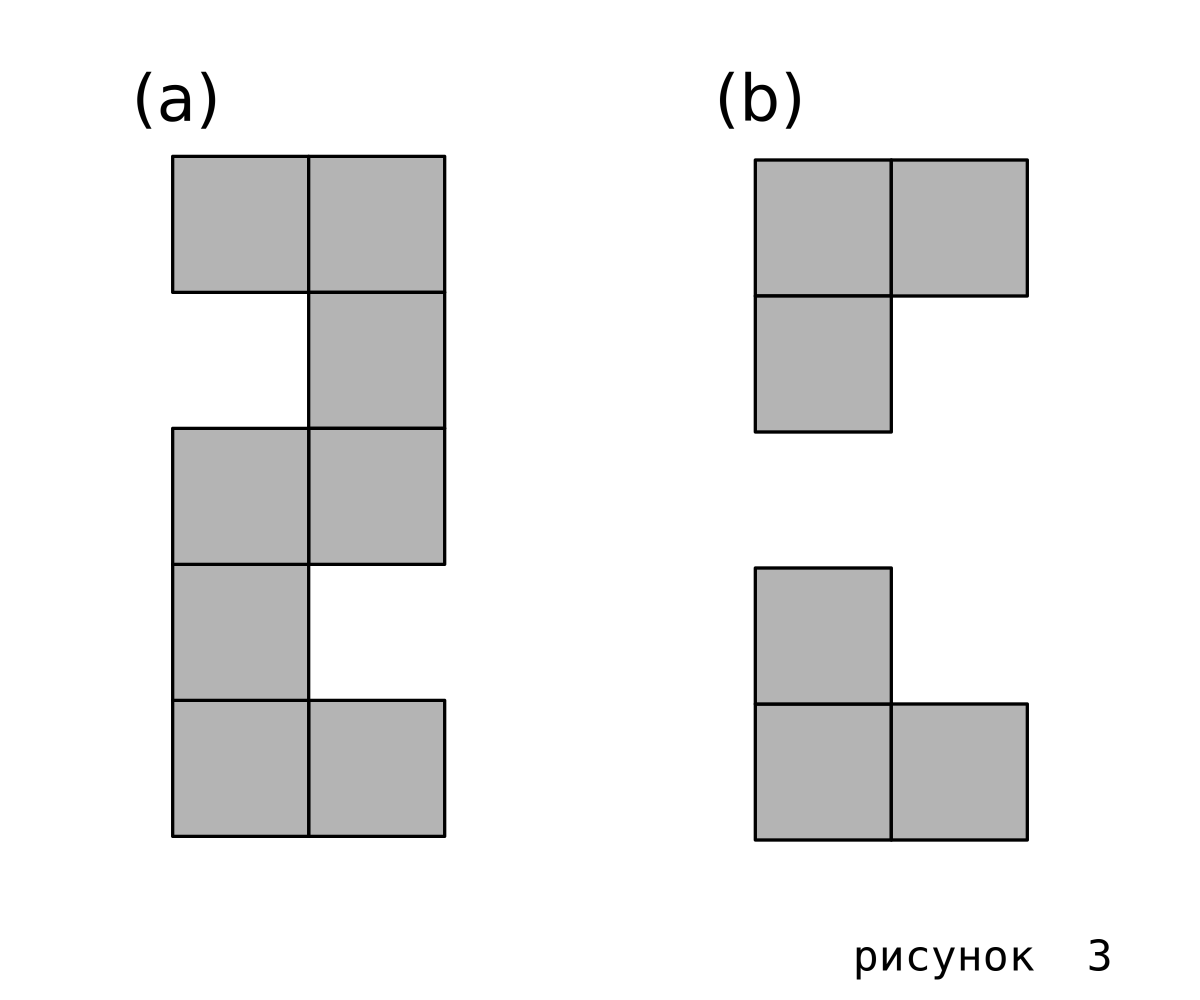
\includegraphics[width=5.5cm]{stats/2018/images/geo-games}}

\itB Клетки прямоугольника $1 \times 303$ пронумерованы от 1 до 303 слева направо. В клетке №2 стоит фишка первого игрока, а в клетке №1~— второго игрока. Каждый игрок может делать ходы двух типов:
	\subitem $*$ из клетки под номером $k$ в клетку $k+1$, если там не стоит фишка другого игрока\scolon
	\subitem $*$ из клетки под номером $k$ в клетку $k+2m$, если $m$~— натуральное число, и в клетке номер $k+m$ сейчас стоит фишка другого игрока (то есть, фишку соперника можно «перепрыгнуть»). \smallskip \\
Выигрывает тот, чья фишка первой окажется в клетке №\,303. У кого из игроков есть выигрышная стратегия?

\itC Двое по очереди вырезают из клетчатого квадрата $4 \times 4$ уголки из трёх клеток, причём первый может вырезать только уголки, ориентированные как буква Г, а второй~— только уголки, ориентированные как буква L (см.\,рис.\,3{\itshape (b)}). Проигрывает тот, кто не может вырезать очередной уголок. У кого из игроков есть выигрышная стратегия?
\end{enumerate}